\section{Anhang} \label{sec:anhang}


\subsection{Elektrotechnik} \label{subsec:eltech}

\subsection{Schaltungsaufbau} \label{subsec:schaltungsaufbau}
(Grundschaltung erklären)
\subsubsection{Parasitäre Paramter}\label{subsec:parasitparam}
In diesem Unterkapitel werden grundsätzlich die Einflüsse und Eigenschaften von Parasitären Paramentern in Realen Bauteilen, besonders Spule und Kondensator, erklärt.

Ideale Bauteile beschreiben eine Funktion. Da reale Bauteile aus Materialien mit physikalischen Eigenschaften bestehen, treten bei der Umsetzung dieser Funktion Nebeneffekte auf. Sie entstehen, weil die einzelnen Bauteile im Betrieb elektrische Felder oder Magnetfelder erzeugen. Oder einfach durch die Leitfähigkeit eines Materials. Diese physikalisch bedingten Effekte werden als parasitär bezeichnet. Sie treten als Widerstand, Induktivität oder Kapazivität auf. Da sie gut klassifiziert werden können, werden sie als Parameter bezeichnet. 
Um eine Schaltung präzise zu simulieren ist es unerlässlich, die elektrischen Bauelemente mit den passenden parasitären Parametern zu ergänzen. In den Abbildungen \ref{fig:stray_L} und \ref{fig:stray_C} werden die parasitären Parameter von Spule und Kondensator gezeigt. Man stellt sie als zusätzliche Bauteile dar. \textcolor{red}{\textbf{TODO:Quelle ganzes kapitel}}


\begin{figure}[H]
	\begin{minipage}[h]{0.45\linewidth}
		\centering
		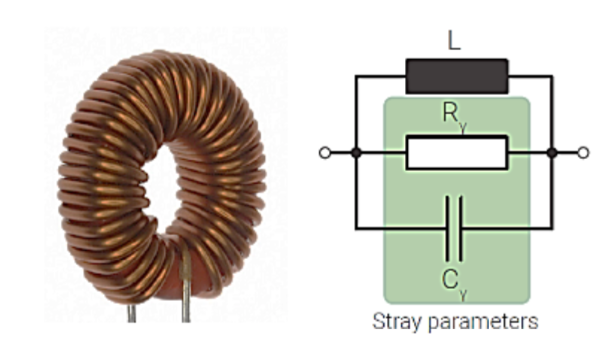
\includegraphics[width = 5cm]{stray_L.png}
		\caption{Parasiäre Elemente einer Induktivität \cite{aufgabenstellung}}
		\label{fig:stray_L}
	\end{minipage}	
	\begin{minipage}[h]{0.45\linewidth}
		\centering
		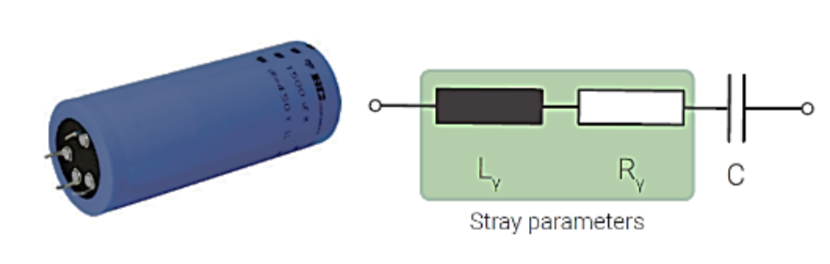
\includegraphics[width = 7cm]{stray_C.png}
		\caption{Parasiäre Elemente einer Kapazität \cite{aufgabenstellung}}
		\label{fig:stray_C}
	\end{minipage}
\end{figure}

\bigskip

\subsubsection{Gleichtakt} \label{subsec:gleichtakt}
In diesem Kapitel ist Schritt für Schritt beschrieben, wie die Gleichtaktschaltung aus der Aufgabenstellung vereinfacht wird. Abbildung \ref{fig:orig_CMSchaltung} zeigt die Schaltung aus der Aufgabenstellung. Diese Schaltung ist mit den Komponenten $R_w$ und $L_r$ ergänzt worden, sodass sie symmetrisch ist(siehe Abbildung \ref{fig:CMSchaltung1}). Dies macht es möglich, dass die Schaltung zur Simulation wie folgt vereinfacht werden kann.
\begin{figure}[H]
	\centering
	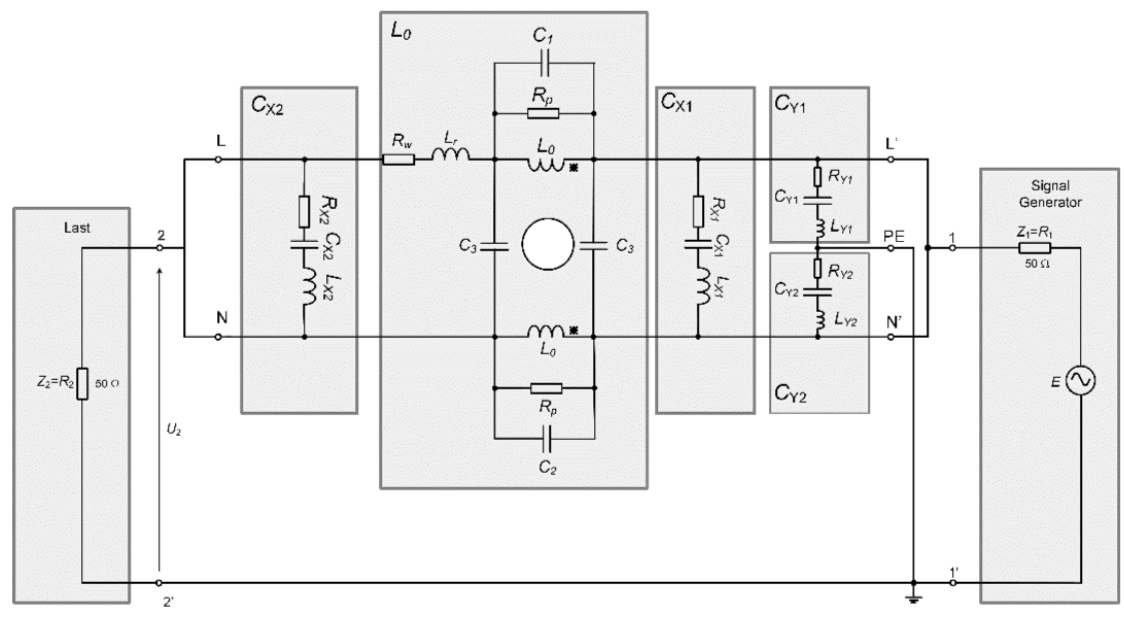
\includegraphics[width = 10cm]{CM_Aufgabenstellung.png}
	\caption{Originale Gleichtaktschaltung\cite{aufgabenstellung}}
	\label{fig:orig_CMSchaltung}
\end{figure}
\begin{figure}[H]
	\centering
	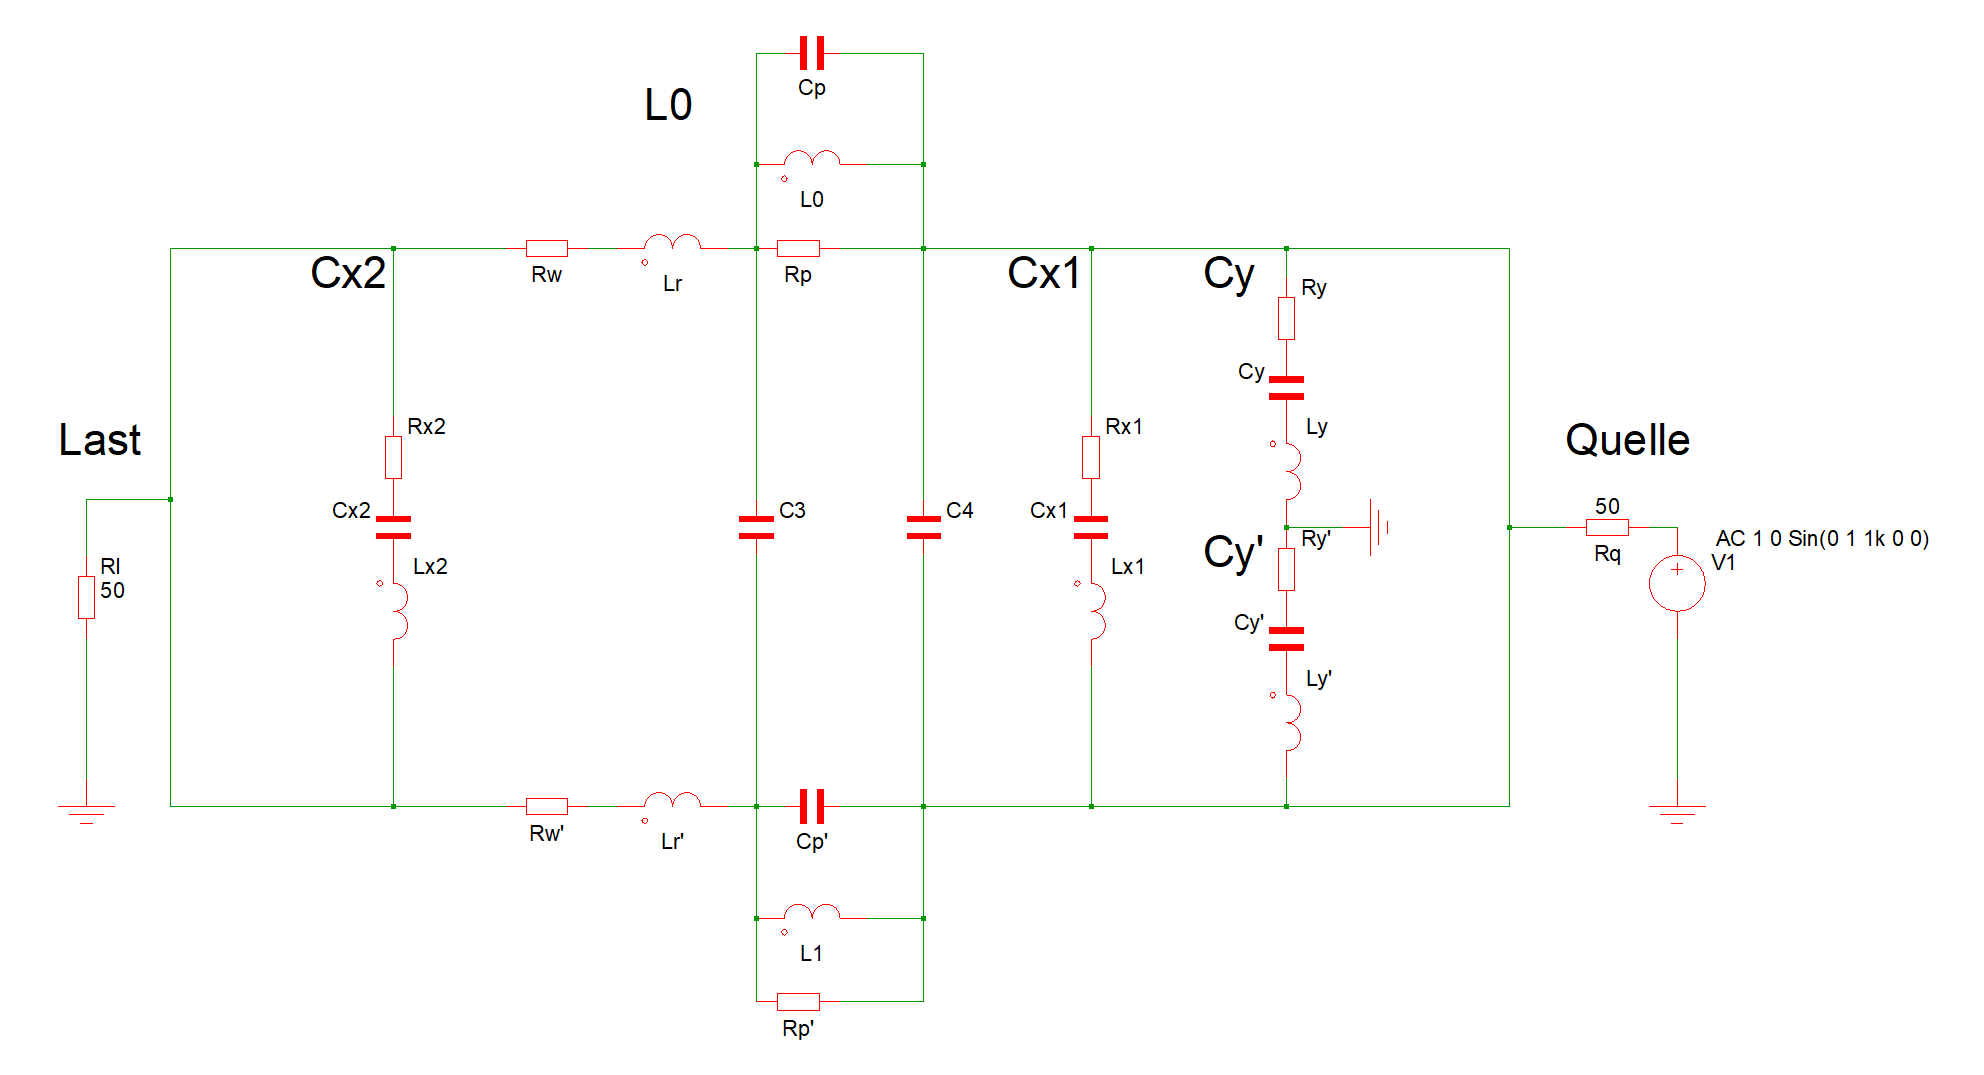
\includegraphics[width = 10cm]{EMI_CMpretty1.png}
	\caption{Ergänzte Gleichtaktschaltung}
	\label{fig:CMSchaltung1}
\end{figure}
Da der obere und untere Strang identisch sind und es keinen Potentialunterschied zwischen ihnen gibt, kann die Schaltung, wie folgt, zusammen gefasst werden (siehe Abbildung \ref{fig:CMSchaltung2}). Die Schaltung wird entlang der Symmetrie-Achse aufgetrennt. Somit fallen die Kondensatoren $C_3$, $C_4$, $C_{x1}$ und $C_{x2}$ komplett weg. Die übrigen Komponenten von $L_0$ bilden eine Parallelschaltung, welche sich durch halbieren der Widerstände und Induktivitäten und verdoppeln der Kapazitäten zusammenfassen lässt. Zusätzlich werden die beiden $C_y$ und $C'_{y}$ parallel auf das Bezugspotential geschalten. Da $C_y$ und $C'_y$ identisch sind, werden sie wie in Abbildung \ref{fig:CMSchaltung2} zusammengefasst. Diese vereinfachte Schaltung bildet die Grundlage für die Berechnungen der Software.
\begin{figure}[H]
	\centering
	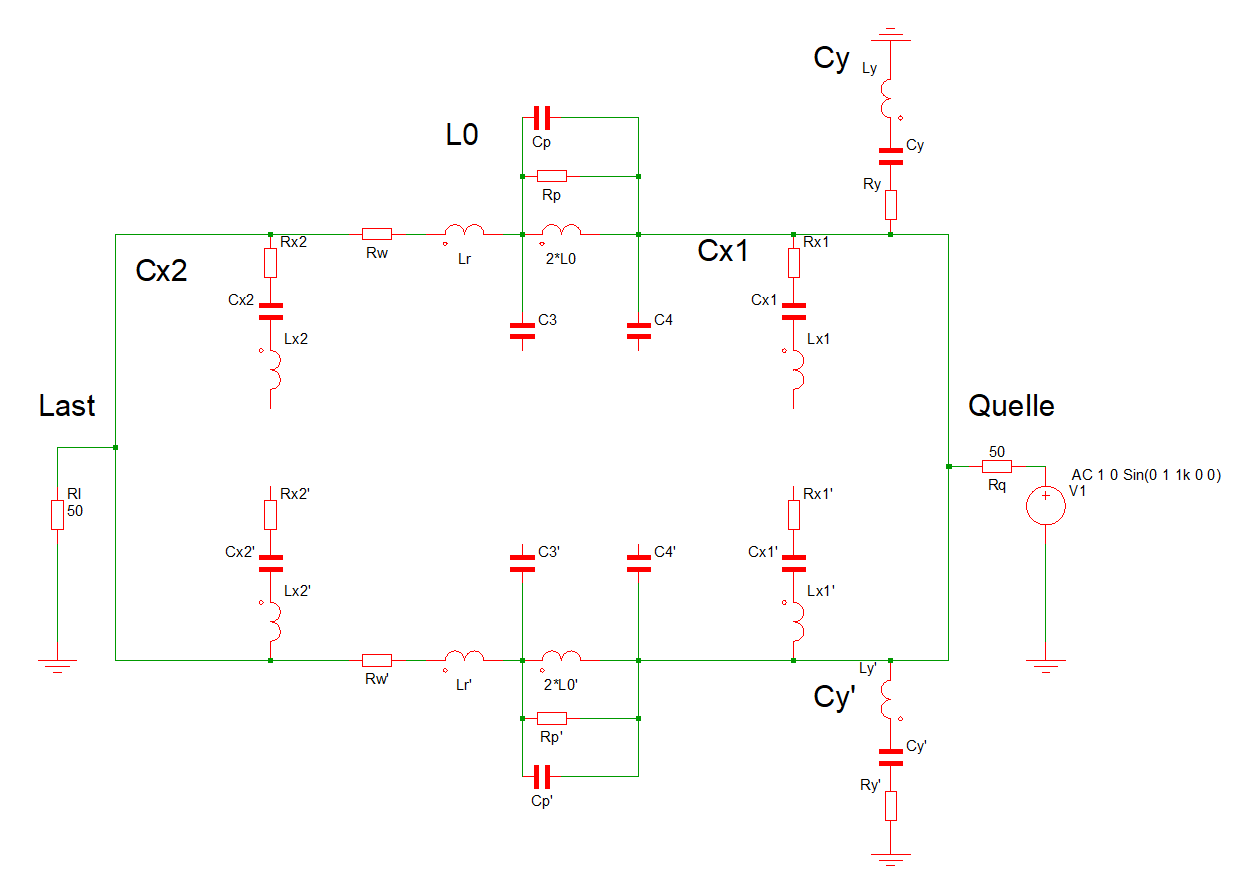
\includegraphics[width = 10cm]{EMI_CMpretty2.png}
	\caption{Vereinfachte Gleichtaktschaltung}
	\label{fig:CMSchaltung2}
\end{figure}
\subsubsection{Gegentakt} \label{subsec:gegentakt}
Beschreibung Differential-Mode und wie man ihn ausrechnet
\subsubsection{Einfügedämpfung}\label{subsec:einfuge}


 Um die Einfügungsverluste bestimmen zu können, wird das Model der 2-Tore verwendet. Einzelne Schaltungsteile werden in ABCD-Matrizen \ref{ABCD-Matrix} abgebildet, welche dann durch Kaskadierung der einzelnen ABCD-Matrixen zusammengeführt werden. Die Einfügungsverluste werden aus den Streuparameter\ref{subsec:Streuparameter} abgeleitet, welche direkt aus der ABCD-Matrix berechnet werden.




\subsubsection{Kettenmatrix}\label{subsubsec:kettenmatrix}
Folgendes Kapitel erklärt die Grundlagen der Kettenmatrix. Die Grundlagen basieren auf den Quellen \cite{hftech}\cite{Bernstein2015}.
Die Kettenmatrix ist eine Variante, um das Verhalten von 2-Toren zu beschreiben. Andere Varianten sind die Z-Matrix oder die Y-Matrix. Die Kettenmatrix hat jedoch den Vorteil, dass man in Serie geschaltene 2-Tore ohne grossen Aufwand zusammen rechnen kann. Sobald man die einzelnen Kettenmatrizen gebildet hat und die Schaltung soweit vereinfacht ist, dass nur noch in Serie geschaltene Ketten-Matrizen vorzufinden sind, können diese miteinander multipliziert werden. Das Matrix-Produkt stellt dann die Kettenmatrix der Gesamtschaltung dar. Folgende gängige Schaltungen helfen, die Kettenmatrizen der einzelnen Schaltungsteilen zu bilden (siehe Anhang: 2-Tor Tabellen).

Die Längsimpedanz lässt sich anhand der Kettenmatrix A\textsubscript{L} (Formel \ref{equ:horizImpedance}) darstellen
\begin{figure}[H]
	\begin{minipage}[h]{0.45\linewidth}
		\centering
		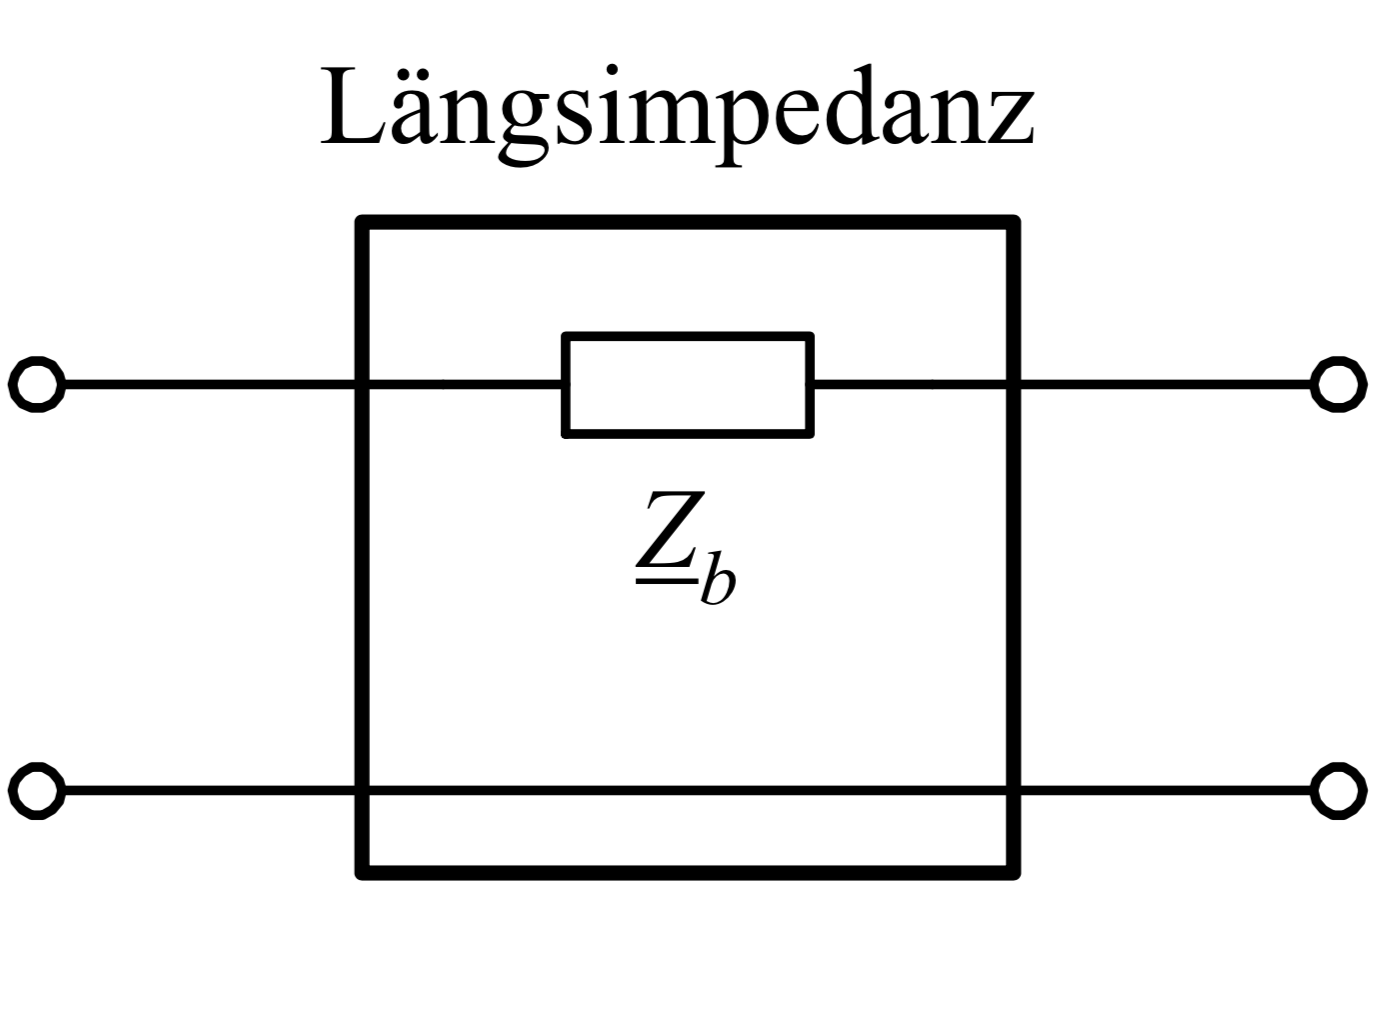
\includegraphics[width = 3cm]{h_impedance.png}
		\caption{Längsimpedanz \ref{sec:anhang}}
	\end{minipage}
	\begin{minipage}[h]{0.45\linewidth}
		\centering
		\begin{equation}\label{equ:horizImpedance}
			A_L = \left[\begin{matrix}
			1&\underline{Z}_b\\0&1
			\end{matrix}\right]
		\end{equation}
	\end{minipage}
\end{figure}

Die Querimpedanz lässt sich anhand der Kettenmatrix A\textsubscript{Q} (Formel \ref{equ:verticImpedance}) darstellen

\begin{figure}[H]
	\begin{minipage}[h]{0.45\linewidth}
		\centering
		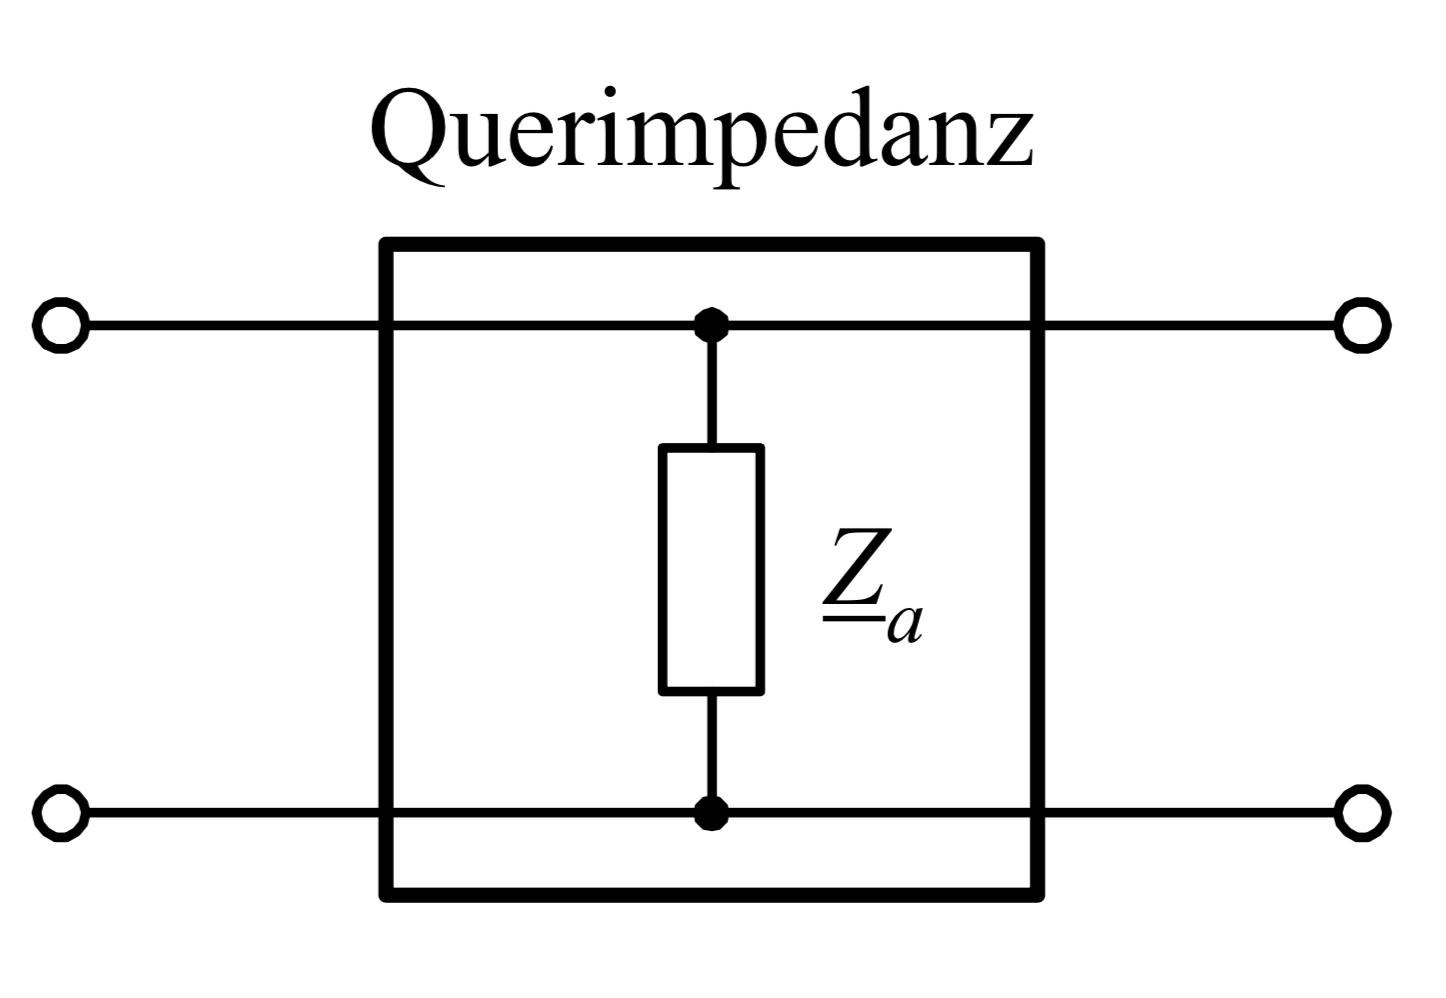
\includegraphics[width = 3cm]{v_impedance.png}
		\caption{Querimpedanz \ref{sec:anhang}}
	\end{minipage}
	\begin{minipage}[h]{0.45\linewidth}
		\centering
		\begin{equation}\label{equ:verticImpedance}
			A_Q = \left[\begin{matrix}
			1&0\\\frac{1}{\underline{Z}_a}&1
			\end{matrix}\right]
		\end{equation}
	\end{minipage}
\end{figure}


Sobald die Kettenmatrix einer Schaltung gebildet wurde, kann diese direkt in die Streuparameter umgewandelt werden. Der $s_{21}$ Parameter kann wie in Formel \ref{equ:s21} beschrieben, durch Einsetzen der Kettenmatrix bestimmt werden. Für den Widerstand $R_w$ muss die verwendete Bezugsimpedanz eingesetzt werden.
\begin{equation}\label{equ:s21}
s_{21} = \frac{2}{A_{11}+\frac{A{12}}{R_w}+A_{21}*R_w+A_{22}}
\end{equation}
Die Indexierung der Kettenmatrix wird in der Formel \ref{equ:A_index} gezeigt.
\begin{equation}\label{equ:A_index}
	A = \left[\begin{matrix}
	A_{11}&A_{12}\\A_{21}&A_{22}
	\end{matrix}\right]
\end{equation}
\newpage


\subsection{Programmieren} \label{subsec:softech}
\subsubsection{MVC-Struktur}\label{subsec:mvc}

Das MVC-Framework wird zur Softwarestrukturierung verwendet. Durch diese Strukturierung werden die Berechnungen der Daten (eng. model), die Steuerung (engl. controller) und dessen graphischer Repräsentation (engl. view) getrennt. In der Abbildung (TODO) ist dieser Aufbau in einem Beispielklassendiagramm dargestellt.

%TODO Bild Gut MVC

Der Ablauf dieser Struktur ist wie folgt: 

\begin{enumerate}
\item Benutzereingabe löst Event aus
\item Die Aktion wird dem Controller übergeben. Dieser holt die Daten in der View, leitet diese dem Model weiter und löst die Berechnungen aus
\item Das Model führt die Berechnungen aus und informiert den Observer
\item Das Model führt die Berechnungen aus und informiert den Observer
\item Der Observer löst ein Event in der View aus. View kann die Daten vom Model holen und Ausgeben
\end{enumerate}



\subsection{Testkonzept} \label{subsec:eltech}


\begin{figure}[H]
	\centering
	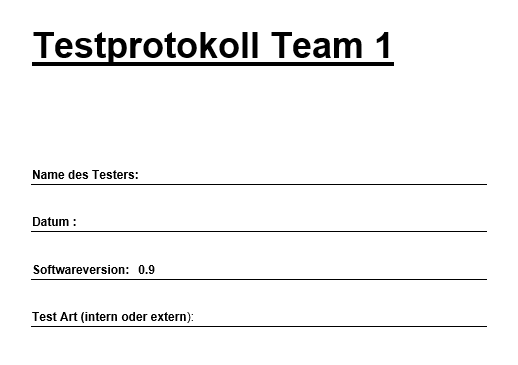
\includegraphics[width=16cm]{Protokoll.png}
	\label{fig:Protokoll}
\end{figure}

\begin{figure}[H]
	\centering
	\includegraphics[width=16cm]{übersicht.png}
	\label{fig:übersicht}
\end{figure}

\begin{figure}[H]
	\centering
	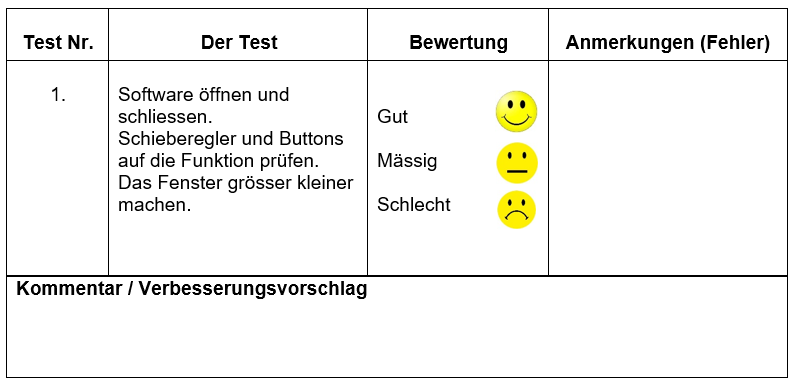
\includegraphics[width=16cm]{Test1.png}
	\label{fig:Test1}
\end{figure}

\begin{figure}[H]
	\centering
	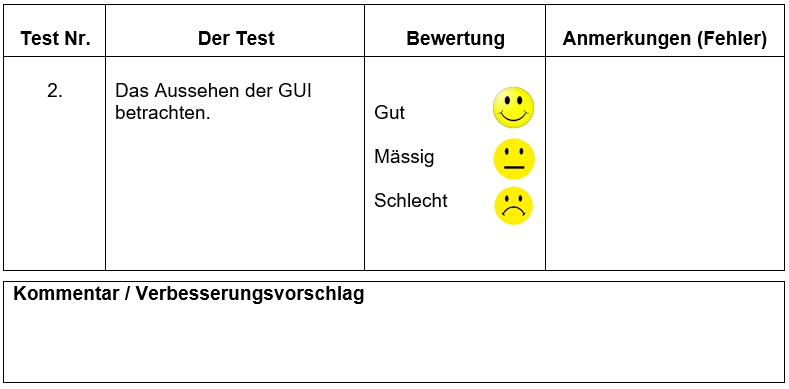
\includegraphics[width=16cm]{Test2.png}
	\label{fig:Test2}
\end{figure}

\begin{figure}[H]
	\centering
	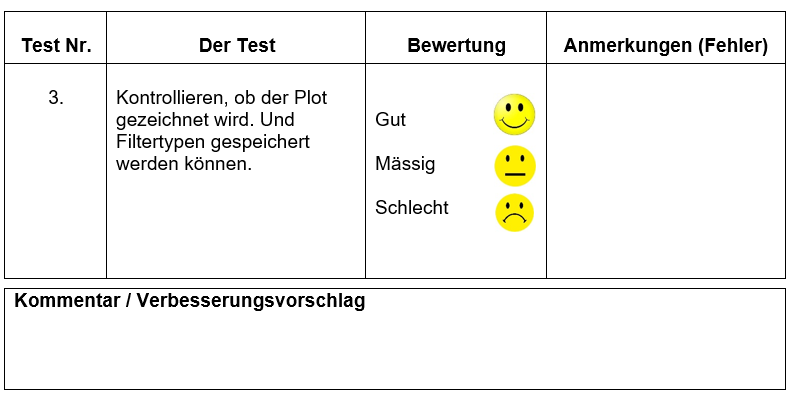
\includegraphics[width=16cm]{Test3.png}
	\label{fig:Test3}
\end{figure}

\begin{figure}[H]
	\centering
	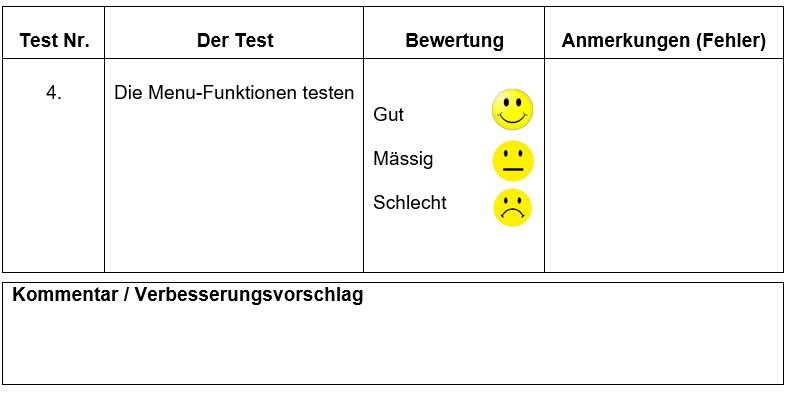
\includegraphics[width=16cm]{Test4.png}
	\label{fig:Test4}
\end{figure}

\begin{figure}[H]
	\centering
	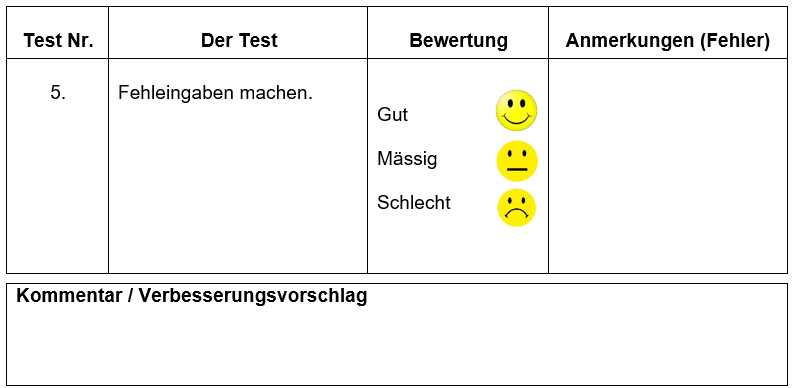
\includegraphics[width=16cm]{Test5.png}
	\label{fig:Test5}
\end{figure}

\begin{figure}[H]
	\centering
	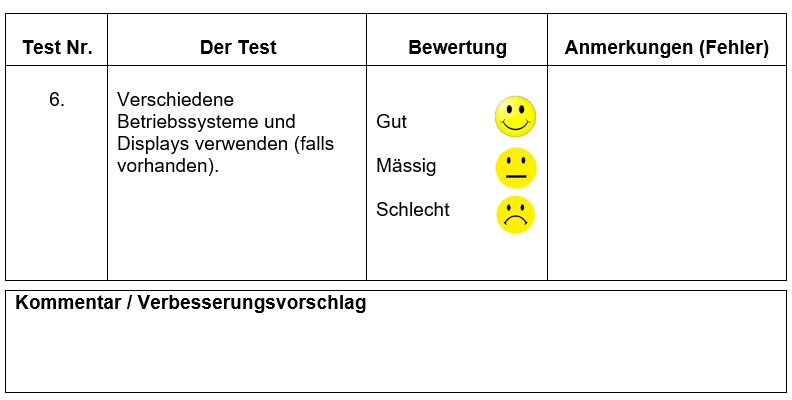
\includegraphics[width=16cm]{Test6.png}
	\label{fig:Test6}
\end{figure}

\begin{figure}[H]
	\centering
	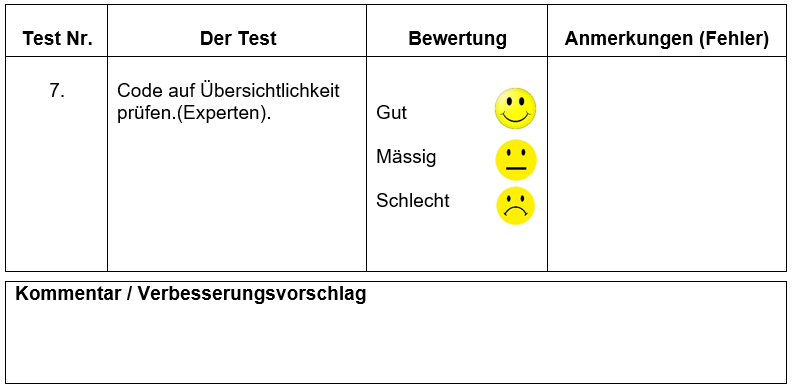
\includegraphics[width=16cm]{Test7.png}
	\label{fig:Test7}
\end{figure}
